\documentclass{beamer}

% Theme élégant
\usetheme{Madrid}
\usecolortheme{seahorse}

% Packages
\usepackage[utf8]{inputenc}
\usepackage[french]{babel}
\usepackage{graphicx}
\usepackage{amsmath}
\usepackage{booktabs}
\usepackage{array}

% Infos
\title[Classification Income Group]{Classification des Revenus des Pays \\ par k-NN}
\author{INF372 - Apprentissage Supervisé et Non Supervisé \\ \textbf{Groupe 1}}
\institute{Université de Yaoundé 1 \\ Département d'Informatique}
\date{Mars 2026}

\begin{document}

% ======================
% SLIDE TITRE
% ======================
\begin{frame}
\titlepage
\end{frame}

% ======================
% MEMBRES DU GROUPE
% ======================
\begin{frame}{Membres du Groupe 1}
\centering
\vspace{0.4cm}
\begin{tabular}{>{\bfseries}l c}
\toprule
\textbf{Nom et Prénom(s)} & \textbf{Matricule} \\
\midrule
MABENGUE BEBONSU JUNIOR Prince   & 22T2832 \\[0.4cm]
ETONDE MABONGO ULRICH Edouard    & 22U2163 \\[0.4cm]
FONAYEN CHRISTIAN Asangwa        & 23V2370 \\
\bottomrule
\end{tabular}
\end{frame}

% ======================
% SOMMAIRE
% ======================
\begin{frame}{Sommaire}
\tableofcontents
\end{frame}

% ======================
% PARTIE I
% ======================

\section{Présentation du Projet}

\begin{frame}{Objectif du Projet}
\begin{itemize}
\item Prédire la catégorie de revenu d'un pays
\item Variable cible : \textbf{Income\_Group}
\item Données : \textbf{1516 indicateurs économiques}
\item Source : Banque Mondiale (année 2023)
\item Algorithme : \textbf{k-Plus Proches Voisins (k-NN)}
\end{itemize}
\end{frame}

% ======================
% PARTIE I — Construction et pretraitement de donnees
% ======================
% Slide de transition
\begin{frame}{}
\centering
\vspace{1.2cm}
{\usebeamerfont{title}\usebeamercolor[fg]{title} Partie I}\\[0.5cm]
{\Large \textbf{Construction et pretraitement de donnees}}\\[0.3cm]
\rule{0.5\textwidth}{0.4pt}
\end{frame}
% ======================
\section{Construction du Dataset}

\begin{frame}{Construction du Jeu de Données}
\begin{itemize}
\item Téléchargement automatique via API
\item Extraction des fichiers CSV
\item Sélection des valeurs 2023
\item Pivotage : 1 pays = 1 ligne
\item 1516 indicateurs = colonnes
\end{itemize}

\vspace{0.5cm}

\textbf{Dimensions finales :}
\begin{itemize}
\item 216 pays
\item 1516 indicateurs
\item 1 variable cible
\end{itemize}
\end{frame}

\section{Pretraitement des donnees}
\begin{frame}{Problème des Valeurs Manquantes}
\begin{itemize}
\item Beaucoup de valeurs manquantes
\item Indicateurs non disponibles pour certains pays
\item Nécessité d'une stratégie d'imputation
\end{itemize}


\textbf{Objectif :}
\begin{itemize}
\item Préserver la cohérence économique
\item Éviter le biais entre pays riches et pauvres
\end{itemize}

\end{frame}

% ======================
\begin{frame}{Choix : Imputation Stratifiée}
Principe :

\begin{block}{Idée}
Remplacer les valeurs manquantes par la médiane du groupe de revenu
\end{block}

\begin{itemize}
\item Low income avec Low income
\item High income avec High income
\item Pas de mélange des profils économiques
\end{itemize}

\end{frame}

% ======================
\begin{frame}{Pourquoi la Médiane ?}
\begin{itemize}
\item Robuste aux valeurs extrêmes
\item Représente mieux la tendance centrale
\item Évite l'influence des outliers
\end{itemize}

\textbf{Exemple :}

\[
\text{Moyenne} \neq \text{Médiane}
\]

La médiane est plus stable pour les données économiques.

\end{frame}

% ======================
\begin{frame}{Illustration Imputation}
\centering
% ESPACE IMAGE
\includegraphics[width=0.8\textwidth]{Screenshot from 2026-03-28 17-50-48.png}

\small{Imputation par groupe de revenu}
\end{frame}

% ======================
% PARTIE II — ANALYSE STATISTIQUE
% ======================
\section{Analyse Statistique}

% Slide de transition
\begin{frame}{}
\centering
\vspace{1.2cm}
{\usebeamerfont{title}\usebeamercolor[fg]{title} Partie II}\\[0.5cm]
{\Large \textbf{Analyse Statistique}}\\[0.3cm]
\rule{0.5\textwidth}{0.4pt}
\end{frame}

\begin{frame}{1. Nettoyage et Filtrage des Données}
    \begin{itemize}
        \item \textbf{Seuil de complétude :} Suppression des indicateurs avec $>50\%$ de valeurs manquantes.
        \item \textbf{Variance Nulle :} Élimination des colonnes constantes
        \item \textbf{Résultat :} Réduction de 1518 à 1132 indicateurs pertinents.
    \end{itemize}
\end{frame}

\begin{frame}{2. Stratégie d'Imputation}
    \begin{itemize}
        \item \textbf{Approche :} Imputation par la médiane au sein de chaque groupe de revenu.
        \item \textbf{Justification :} Moins sensible aux valeurs extrêmes que la moyenne.
        \item \textbf{Finalisation :} Médiane globale pour les cas résiduels afin d'assurer un dataset complet pour le k-NN.
    \end{itemize}
\end{frame}

\begin{frame}{3. Découpage Train/Test}
    \begin{itemize}
        \item \textbf{Répartition :} 80\% Entraînement / 20\% Test.
        \item \textbf{Stratification :} Maintien des proportions de chaque classe (High, Upper-Middle, Lower-Middle, Low).
        \item \textbf{Stabilité :} Garantit que l'évaluation reflète la réalité du dataset déséquilibré.
    \end{itemize}
\end{frame}

\begin{frame}{4. Standardisation (Z-Score)}
    \begin{itemize}
        \item \textbf{Formule :} $z = \frac{x - \mu_{train}}{\sigma_{train}}$.
        \item \textbf{Objectif :} Ramener tous les indicateurs à la même échelle (Moyenne 0, Écart-type 1).
        \item \textbf{Impact k-NN :} Évite que les variables à fortes unités ne dominent le calcul de distance.
    \end{itemize}
\end{frame}

%======================
% PARTIE III — Definition des distances et implementation du k-NN
% ======================
\section{Definition des distances et implementation du k-NN}

% Slide de transition
\begin{frame}{}
\centering
\vspace{1.2cm}
{\usebeamerfont{title}\usebeamercolor[fg]{title} Partie III}\\[0.5cm]
{\Large \textbf{Definition des distances et implementation du k-NN}}\\[0.3cm]
\rule{0.5\textwidth}{0.4pt}
\end{frame}

\begin{frame}{1. Calcul de la distance}
    \begin{itemize}
        \item \textbf{Distance euclidienne :} $d(x,y) = \sqrt{\sum_{i=1}^{n} (x_i - y_i)^2}$
        \item \textbf{Resultat du test :} $19.3294$
        \item \textbf{Distance de Manhattan :} $d(x,y) = \sum_{i=1}^{n} |x_i - y_i|$
        \item \textbf{Resultat du test :} $263.6925$
        \item \textbf{Distance de Minkowski :} $d(x,y) = \left( \sum_{i=1}^{n} |x_i - y_i|^p \right)^{1/p}$
        \item \textbf{Resultat du test :} $9.1850$ pour $p=3$ et $5.6303$ pour $p=5$
    \end{itemize}
\end{frame}

\begin{frame}{2. Visualisation des distances}
\centering
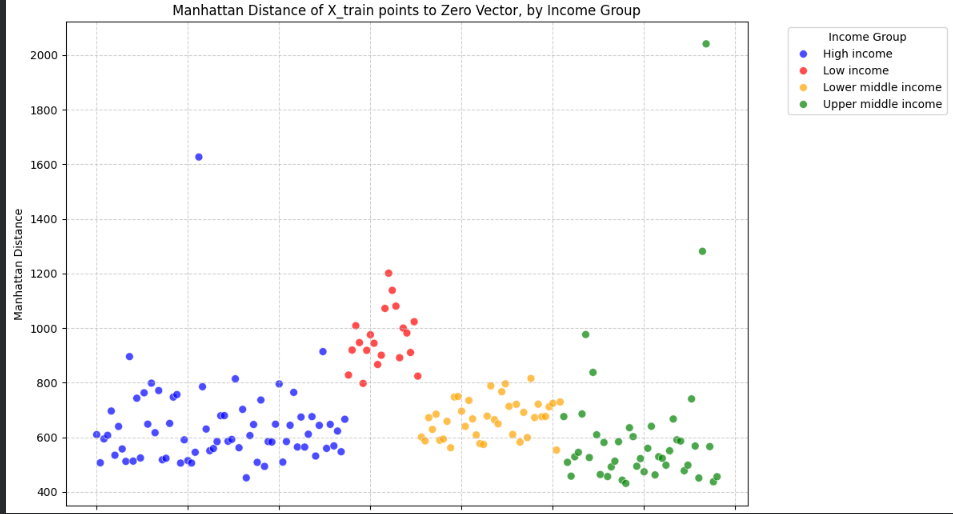
\includegraphics[width=0.82\textwidth]{training-points.png}
\vspace{0.2cm}

\small{Visualisation des points d'entrainement}
\end{frame}

\begin{frame}{3. Algorithme k-NN}
    \begin{itemize}
        \item L'algorithme \textbf{k-Nearest Neighbors (k-NN)} est implemente de maniere personnalisee.
        \item \texttt{\_\_init\_\_(k=3)} : initialise le modele avec un nombre de voisins $k$.
        \item \texttt{fit(X, y)} : stocke les donnees d'entrainement (\texttt{Xtrain}) et les labels (\texttt{ytrain}).
        \item \texttt{predict(new\_points)} : predit les labels de plusieurs points en appelant \texttt{predict\_class}.
        \item \texttt{predict\_class(new\_point)} :
        \begin{enumerate}
            \item calcule la distance entre le nouveau point et tous les points d'entrainement avec la distance de Minkowski ($p=5$) ;
            \item trie les distances et selectionne les indices des $k$ plus proches voisins ;
            \item recupere les labels des voisins ;
            \item applique un vote majoritaire (via \texttt{Counter}) pour retourner la classe la plus frequente.
        \end{enumerate}
    \end{itemize}
\end{frame}

\begin{frame}{4. Evaluation de la precision}
    \begin{itemize}
        \item Precision observee : \textbf{100\%}
    \end{itemize}
\centering
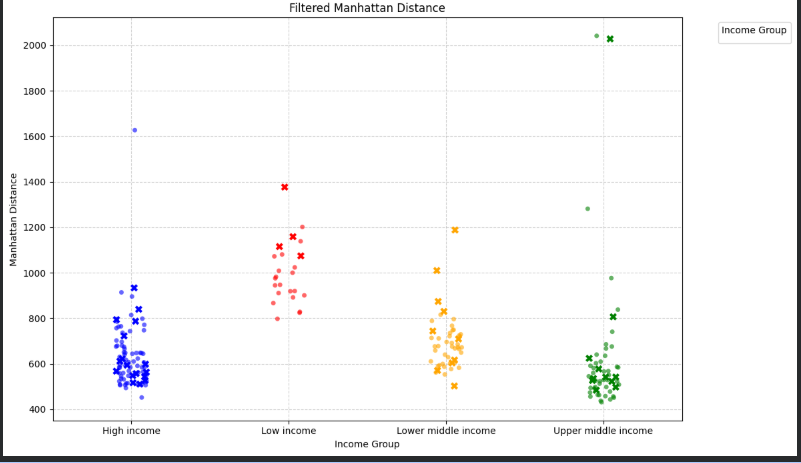
\includegraphics[width=0.82\textwidth]{predicted-points.png}
\vspace{0.2cm}

\small{Visualisation des points predits}
\end{frame}

\end{document}